\documentclass{standalone}
\usepackage{pgfplots}
\pgfplotsset{compat=1.5}
\usepgfplotslibrary{fillbetween}
\usetikzlibrary{shapes,positioning,intersections,quotes,patterns}

\pgfplotsset{soldot/.style={color=black,only marks,mark=*}} 
\pgfplotsset{holdot/.style={fill=white,mark=*}}

\begin{document}

\centering
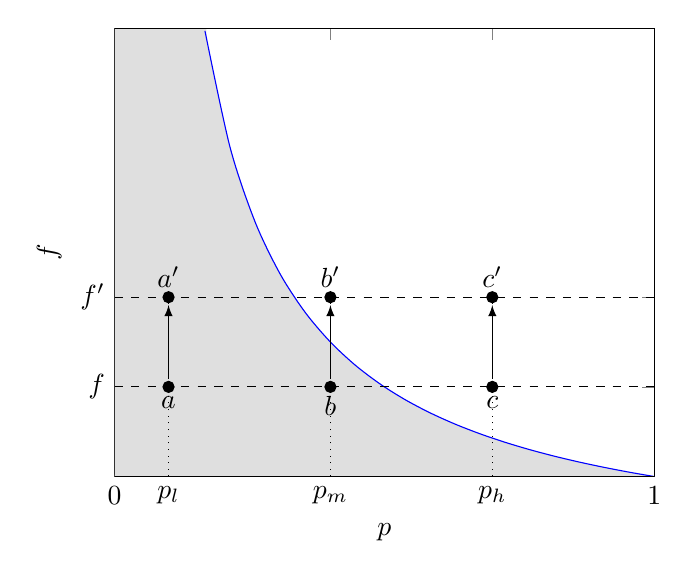
\begin{tikzpicture}
\begin{axis}[
xlabel={$p$},
ylabel={$f$},
smooth,
%legend style={draw=none}
xmin=0,
xmax=1,
ymin=0,
ymax=5,
ytick={1,2},
yticklabels={$f$,$f^\prime$},
xtick={0,0.1,0.4,0.7,1},
xticklabels={0,$p_l$,$p_m$,$p_h$,1},
restrict y to domain=0:5,
]

% Plots
\addplot[name path=F,domain=-0.11:1,solid, blue] {1*(1-x)/x};
\addplot[name path=G,black,domain={0:1}] {0};
\addplot[name path=M,black,domain={0:1}] {5};

% Shading
\addplot[fill=gray!25]fill between[of=F and G, soft clip={domain=0:1}];
\addplot[fill=gray!25]fill between[of=M and G, soft clip={domain=0:0.17}];
% Correcting vertical axis that got covered by shade
\draw[] (axis cs:0,0) -- (axis cs:0,5);

% Values of probability of detection
\draw[dotted] (axis cs:0.1,0) -- (axis cs:0.1,2);
\draw[dotted] (axis cs:0.4,0) -- (axis cs:0.4,2);
\draw[dotted] (axis cs:0.7,0) -- (axis cs:0.7,2);

% Fines
\addplot[domain=0:1,dashed,mark=none,black] {1};
\addplot[domain=0:1,dashed,mark=none,black] {2};
\addplot[soldot] coordinates{(0.1,1)} node[below](a) {$a$};
\addplot[soldot] coordinates{(0.4,1)} node[below](b) {$b$};
\addplot[soldot] coordinates{(0.7,1)} node[below](c) {$c$};
\addplot[soldot] coordinates{(0.1,2)} node[above](d) {$a^\prime$};
\addplot[soldot] coordinates{(0.4,2)} node[above](e) {$b^{\prime}$};
\addplot[soldot] coordinates{(0.7,2)} node[above](f) {$c^\prime$};

\draw[>=latex,shorten >=0.1cm,shorten <=0.1cm, black, ->] (a)--(d);
\draw[>=latex,shorten >=0.1cm,shorten <=0.1cm, black, ->] (b)--(e);
\draw[>=latex,shorten >=0.1cm,shorten <=0.1cm, black, ->] (c)--(f);

\end{axis}
\end{tikzpicture}

\end{document}